% Options for packages loaded elsewhere
\PassOptionsToPackage{unicode}{hyperref}
\PassOptionsToPackage{hyphens}{url}
\PassOptionsToPackage{dvipsnames,svgnames,x11names}{xcolor}
%
\documentclass[
  11pt,
]{article}

\usepackage{amsmath,amssymb}
\usepackage{iftex}
\ifPDFTeX
  \usepackage[T1]{fontenc}
  \usepackage[utf8]{inputenc}
  \usepackage{textcomp} % provide euro and other symbols
\else % if luatex or xetex
  \usepackage{unicode-math}
  \defaultfontfeatures{Scale=MatchLowercase}
  \defaultfontfeatures[\rmfamily]{Ligatures=TeX,Scale=1}
\fi
\usepackage{lmodern}
\ifPDFTeX\else  
    % xetex/luatex font selection
\fi
% Use upquote if available, for straight quotes in verbatim environments
\IfFileExists{upquote.sty}{\usepackage{upquote}}{}
\IfFileExists{microtype.sty}{% use microtype if available
  \usepackage[]{microtype}
  \UseMicrotypeSet[protrusion]{basicmath} % disable protrusion for tt fonts
}{}
\makeatletter
\@ifundefined{KOMAClassName}{% if non-KOMA class
  \IfFileExists{parskip.sty}{%
    \usepackage{parskip}
  }{% else
    \setlength{\parindent}{0pt}
    \setlength{\parskip}{6pt plus 2pt minus 1pt}}
}{% if KOMA class
  \KOMAoptions{parskip=half}}
\makeatother
\usepackage{xcolor}
\usepackage[margin=1in]{geometry}
\setlength{\emergencystretch}{3em} % prevent overfull lines
\setcounter{secnumdepth}{-\maxdimen} % remove section numbering
% Make \paragraph and \subparagraph free-standing
\ifx\paragraph\undefined\else
  \let\oldparagraph\paragraph
  \renewcommand{\paragraph}[1]{\oldparagraph{#1}\mbox{}}
\fi
\ifx\subparagraph\undefined\else
  \let\oldsubparagraph\subparagraph
  \renewcommand{\subparagraph}[1]{\oldsubparagraph{#1}\mbox{}}
\fi


\providecommand{\tightlist}{%
  \setlength{\itemsep}{0pt}\setlength{\parskip}{0pt}}\usepackage{longtable,booktabs,array}
\usepackage{calc} % for calculating minipage widths
% Correct order of tables after \paragraph or \subparagraph
\usepackage{etoolbox}
\makeatletter
\patchcmd\longtable{\par}{\if@noskipsec\mbox{}\fi\par}{}{}
\makeatother
% Allow footnotes in longtable head/foot
\IfFileExists{footnotehyper.sty}{\usepackage{footnotehyper}}{\usepackage{footnote}}
\makesavenoteenv{longtable}
\usepackage{graphicx}
\makeatletter
\def\maxwidth{\ifdim\Gin@nat@width>\linewidth\linewidth\else\Gin@nat@width\fi}
\def\maxheight{\ifdim\Gin@nat@height>\textheight\textheight\else\Gin@nat@height\fi}
\makeatother
% Scale images if necessary, so that they will not overflow the page
% margins by default, and it is still possible to overwrite the defaults
% using explicit options in \includegraphics[width, height, ...]{}
\setkeys{Gin}{width=\maxwidth,height=\maxheight,keepaspectratio}
% Set default figure placement to htbp
\makeatletter
\def\fps@figure{htbp}
\makeatother

\usepackage{array}
\usepackage{booktabs}
\usepackage{graphicx}
\usepackage{longtable}
\usepackage{needspace}
\usepackage{caption}
\usepackage{float}
\usepackage{fancyhdr}
\pagestyle{fancy}
\fancyhf{}
\fancyhead[L]{Video Quality Analysis Report}
\fancyhead[R]{Fifth Avenue Studios}
\fancyfoot[L]{\today}
\fancyfoot[C]{\thepage}
\fancyfoot[R]{Gil Raitses}
\setlength{\extrarowheight}{1pt}
\renewcommand{\arraystretch}{1.0}
\makeatletter
\makeatother
\makeatletter
\makeatother
\makeatletter
\@ifpackageloaded{caption}{}{\usepackage{caption}}
\AtBeginDocument{%
\ifdefined\contentsname
  \renewcommand*\contentsname{Table of contents}
\else
  \newcommand\contentsname{Table of contents}
\fi
\ifdefined\listfigurename
  \renewcommand*\listfigurename{List of Figures}
\else
  \newcommand\listfigurename{List of Figures}
\fi
\ifdefined\listtablename
  \renewcommand*\listtablename{List of Tables}
\else
  \newcommand\listtablename{List of Tables}
\fi
\ifdefined\figurename
  \renewcommand*\figurename{Figure}
\else
  \newcommand\figurename{Figure}
\fi
\ifdefined\tablename
  \renewcommand*\tablename{Table}
\else
  \newcommand\tablename{Table}
\fi
}
\@ifpackageloaded{float}{}{\usepackage{float}}
\floatstyle{ruled}
\@ifundefined{c@chapter}{\newfloat{codelisting}{h}{lop}}{\newfloat{codelisting}{h}{lop}[chapter]}
\floatname{codelisting}{Listing}
\newcommand*\listoflistings{\listof{codelisting}{List of Listings}}
\makeatother
\makeatletter
\@ifpackageloaded{caption}{}{\usepackage{caption}}
\@ifpackageloaded{subcaption}{}{\usepackage{subcaption}}
\makeatother
\makeatletter
\@ifpackageloaded{tcolorbox}{}{\usepackage[skins,breakable]{tcolorbox}}
\makeatother
\makeatletter
\@ifundefined{shadecolor}{\definecolor{shadecolor}{rgb}{.97, .97, .97}}
\makeatother
\makeatletter
\makeatother
\makeatletter
\makeatother
\ifLuaTeX
  \usepackage{selnolig}  % disable illegal ligatures
\fi
\IfFileExists{bookmark.sty}{\usepackage{bookmark}}{\usepackage{hyperref}}
\IfFileExists{xurl.sty}{\usepackage{xurl}}{} % add URL line breaks if available
\urlstyle{same} % disable monospaced font for URLs
\hypersetup{
  pdftitle={Video Quality Analysis Report - IMG\_3788.mov},
  colorlinks=true,
  linkcolor={blue},
  filecolor={Maroon},
  citecolor={Blue},
  urlcolor={Blue},
  pdfcreator={LaTeX via pandoc}}

\title{Video Quality Analysis Report - IMG\_3788.mov}
\usepackage{etoolbox}
\makeatletter
\providecommand{\subtitle}[1]{% add subtitle to \maketitle
  \apptocmd{\@title}{\par {\large #1 \par}}{}{}
}
\makeatother
\subtitle{Flaco Owl Documentary Footage - Fifth Avenue Studios}
\author{}
\date{2025-11-13}

\begin{document}
\maketitle
\begin{abstract}
This report analyzes 15.83 seconds of video footage documenting Flaco
the owl's first landing on Fifth Avenue on February 4, 2024, the night
he was freed from the Central Park Zoo. Technical analysis reveals Full
HD resolution (720 × 1280 pixels, 30 fps) with overall quality score of
49.7/100, requiring post-processing for sharpness (33.65) and stability
(5.43), though the footage demonstrates good exposure (98.0/100),
minimal noise (5.32) and high smoothness (0.937). Content analysis using
ML object detection shows the subject (bird/owl) visible in 43.8\% of
analyzed frames (14 of 32 frames), documenting a rare and historic
moment. The footage achieves 100\% usability (15.83 seconds usable) with
43.8\% meeting high-quality standards (6.93 seconds). Narrative
significance scores 100/100 due to the rare/unique event nature,
historic moment value, subject visibility and multiple-use potential
throughout documentary production. Valuation analysis indicates a rate
of \$140.62 per usable second based on base rate (\$50.00) modified by
quality (0.50×), content significance (1.50×), narrative significance
(2.50×) and multiple-use (1.50×) multipliers, resulting in an estimated
value range of \$2,226 - \$2,713. This footage represents an important
moment in Flaco's story with archival and narrative value for
documentary production.
\end{abstract}
\ifdefined\Shaded\renewenvironment{Shaded}{\begin{tcolorbox}[interior hidden, borderline west={3pt}{0pt}{shadecolor}, enhanced, boxrule=0pt, frame hidden, breakable, sharp corners]}{\end{tcolorbox}}\fi

\needspace{8cm}
\section{Executive Summary}

This report provides a technical and narrative analysis of video footage
documenting Flaco the owl's first-night landing on Fifth Avenue after
being freed from the Central Park Zoo. The footage has been evaluated
for documentary production suitability and content significance.

\begin{table}[h]
\centering
\small
\caption{Executive Summary Findings}
\label{tab-exec-summary}
\begin{tabular}{p{3cm}p{8cm}}
\toprule
\textbf{Finding} & \textbf{Value} \\
\midrule
Total Duration & 15.83 seconds \\
Usable Footage & 15.83 seconds (100\%) \\
High Quality Segments & 6.93 seconds (43.8\%) \\
Narrative Significance & 100/100 (high importance) \\
Estimated Value Range & \$2,226 - \$2,713 \\
\bottomrule
\end{tabular}
\end{table}

\begin{figure}[h]
\centering
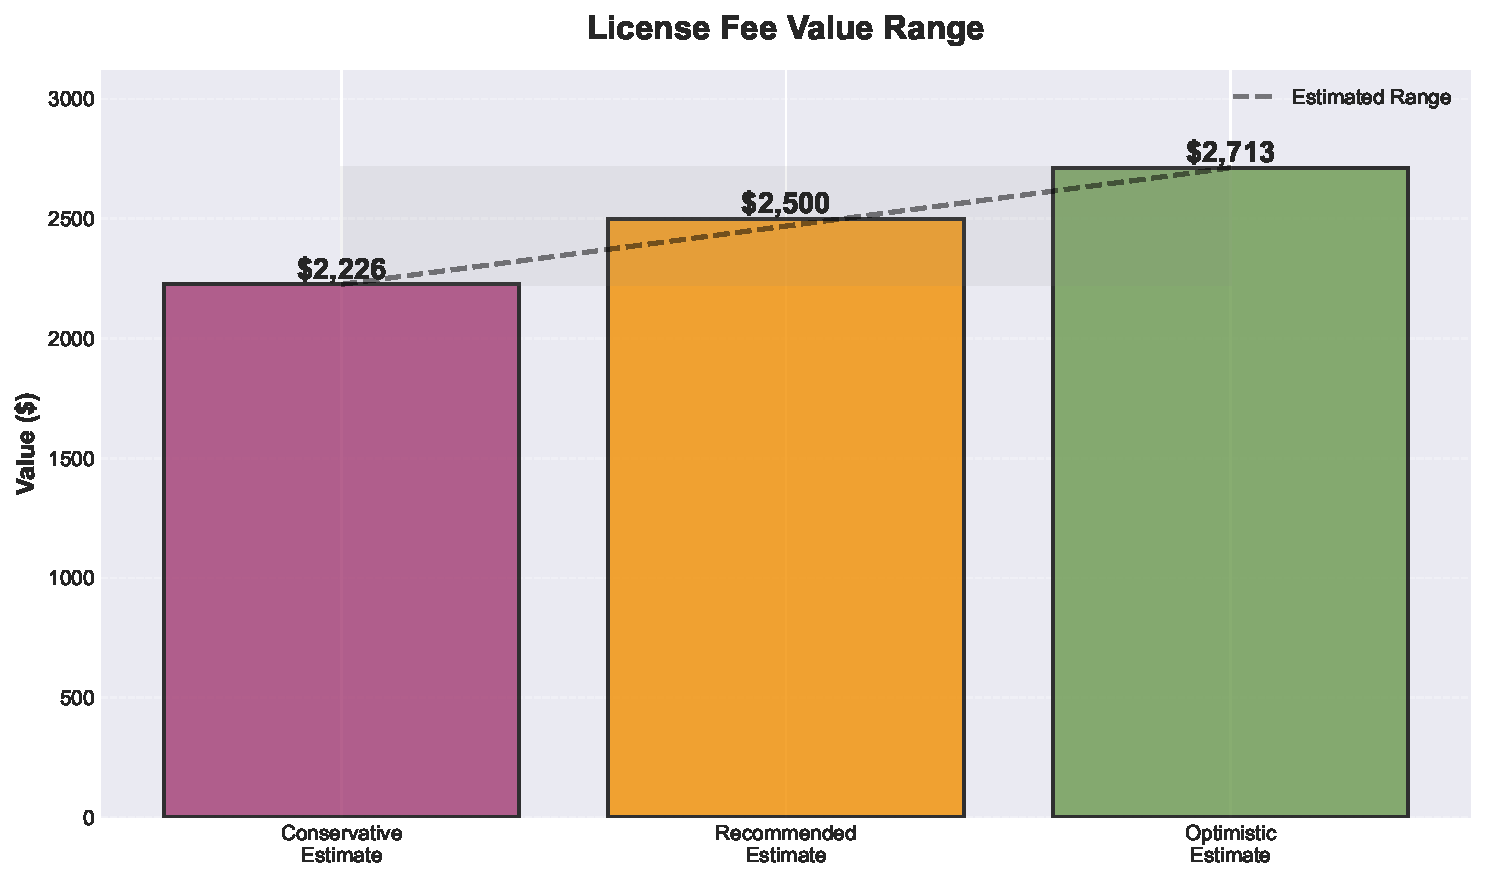
\includegraphics[width=0.85\textwidth]{figures/value_range.pdf}
\caption{Recommended estimate \$2,500 reflects projected fair market value. Bar chart comparing Conservative (\$2,226), Recommended (\$2,500) and Optimistic (\$2,713) valuation estimates.}
\label{fig-value-range}
\end{figure}

\needspace{8cm}
\section{Technical Specifications}

\begin{table}[h]
\centering
\small
\caption{Technical Specifications}
\label{tab-tech-specs}
\begin{tabular}{p{3cm}p{7.5cm}}
\toprule
\textbf{Property} & \textbf{Value} \\
\midrule
File Name & IMG\_3788.mov \\
Resolution & 720 × 1280 pixels (Full HD 1080p, Portrait) \\
Frame Rate & 30.00 fps \\
Duration & 15.83 seconds \\
Total Frames & 475 frames \\
File Size & 4.76 MB \\
File Format & QuickTime (.mov) \\
Video Codec & H.264 (AVC) \\
Color Depth & 8-bit \\
Pixel Format & YUV 4:2:0 \\
Aspect Ratio & 9:16 (Portrait) \\
\bottomrule
\end{tabular}
\end{table}

\needspace{10cm}
\section{Visual Quality Metrics}

\subsection{Core Quality Metrics}

\begin{table}[h]
\centering
\small
\caption{Core Quality Metrics}
\label{tab-quality-metrics}
\begin{tabular}{p{3.5cm}p{2cm}p{5.5cm}}
\toprule
\textbf{Metric} & \textbf{Score} & \textbf{Assessment} \\
\midrule
Sharpness & 33.65 & Very Soft/Blurry \\
Brightness & 72.8/255 & Underexposed \\
Contrast & 44.53 & High Contrast \\
Noise Level & 5.32 & Very Clean \\
Exposure & 98.0/100 & Good Exposure \\
Stability & 5.43 & Unstable/Shaky \\
Smoothness & 0.937 & Very Smooth \\
Color Compression & 0.876 & Minimal Compression \\
\bottomrule
\end{tabular}
\end{table}

\needspace{12cm}
\subsection{Quality Assessment}

\textbf{Strengths:}

\begin{table}[h]
\centering
\small
\caption{Quality Strengths}
\label{tab-strengths}
\begin{tabular}{p{2cm}p{7cm}}
\toprule
\textbf{Strength} & \textbf{Description} \\
\midrule
Resolution & High resolution (Full HD 1080p) suitable for broadcast \\
Exposure & Well-exposed footage with minimal over/under exposure \\
Noise Level & Clean footage with minimal noise (5.32) \\
Smoothness & High temporal smoothness (0.937) \\
Compression & Minimal color compression artifacts (0.876) \\
\bottomrule
\end{tabular}
\end{table}

\textbf{Post-Processing Considerations:}

\begin{table}[h]
\centering
\small
\caption{Post-Processing Requirements}
\label{tab-post-processing}
\begin{tabular}{p{2cm}p{4cm}p{3cm}}
\toprule
\textbf{Issue} & \textbf{Description} & \textbf{Required Action} \\
\midrule
Sharpness & Footage is soft/blurry (sharpness: 33.65) & Requires sharpening \\
Stability & Camera shake present (stability: 5.43) & Requires stabilization \\
\bottomrule
\end{tabular}
\end{table}

\begin{figure}[h]
\centering
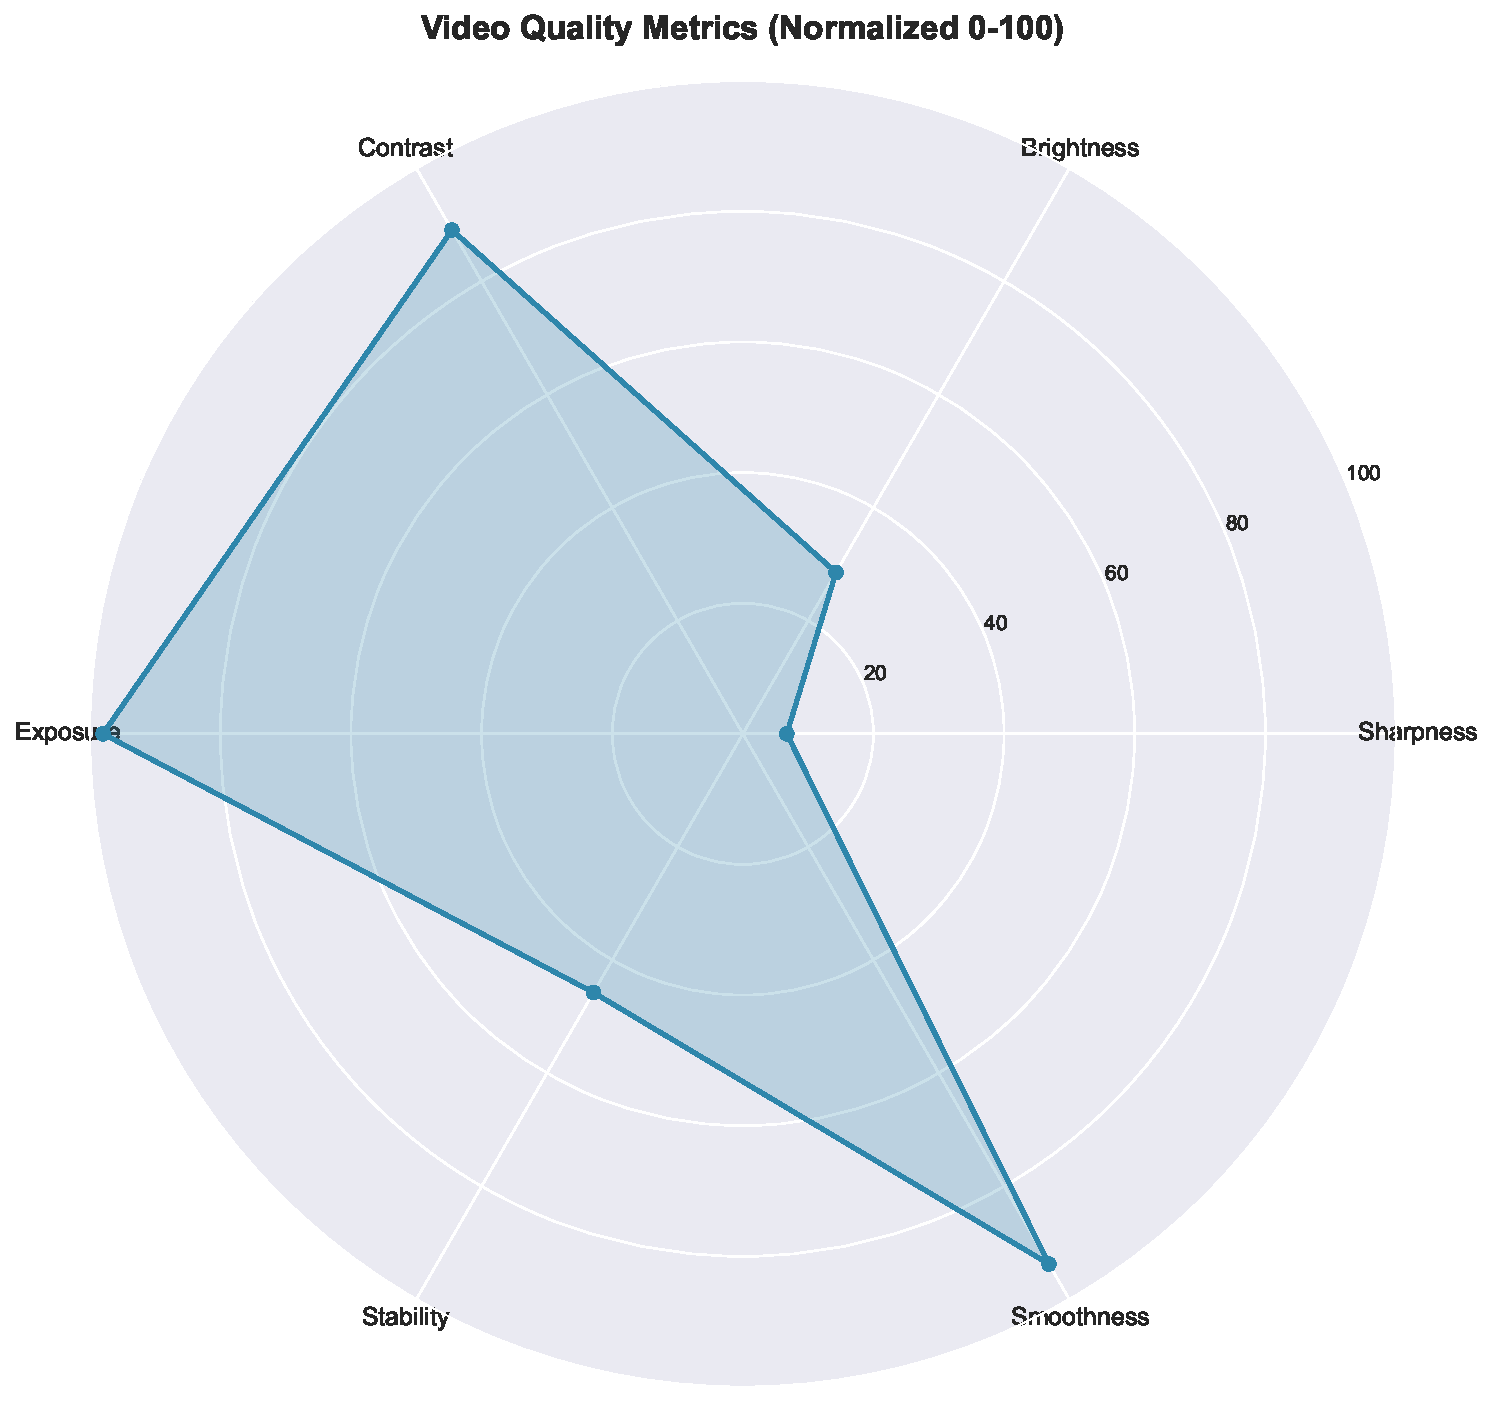
\includegraphics[width=0.7\textwidth]{figures/quality_metrics_radar.pdf}
\caption{Lower scores in sharpness and brightness indicate areas requiring post-processing enhancement. Radar chart showing normalized quality scores across six dimensions: Sharpness (6.7), Brightness (28.5), Contrast (111.3), Exposure (98.0), Stability (45.7) and Smoothness (93.7).}
\label{fig-quality-radar}
\end{figure}

\needspace{22cm}
\section{Content Significance Analysis}

\subsection{Subject Detection}

\begin{table}[h]
\centering
\small
\caption{Subject Detection Metrics}
\label{tab-subject-detection}
\begin{tabular}{p{4.5cm}p{5.5cm}}
\toprule
\textbf{Metric} & \textbf{Value} \\
\midrule
Frames Analyzed & 32 frames \\
Frames with Subject (Bird/Owl) & 14 frames (43.8\%) \\
Frames with Dog & 0 frames \\
Frames with Interaction & 0 frames \\
Subject Visible Throughout & No \\
Interaction Moments Detected & No \\
Rare/Unique Event & Yes \\
\bottomrule
\end{tabular}
\end{table}

\begin{figure}[h]
\centering
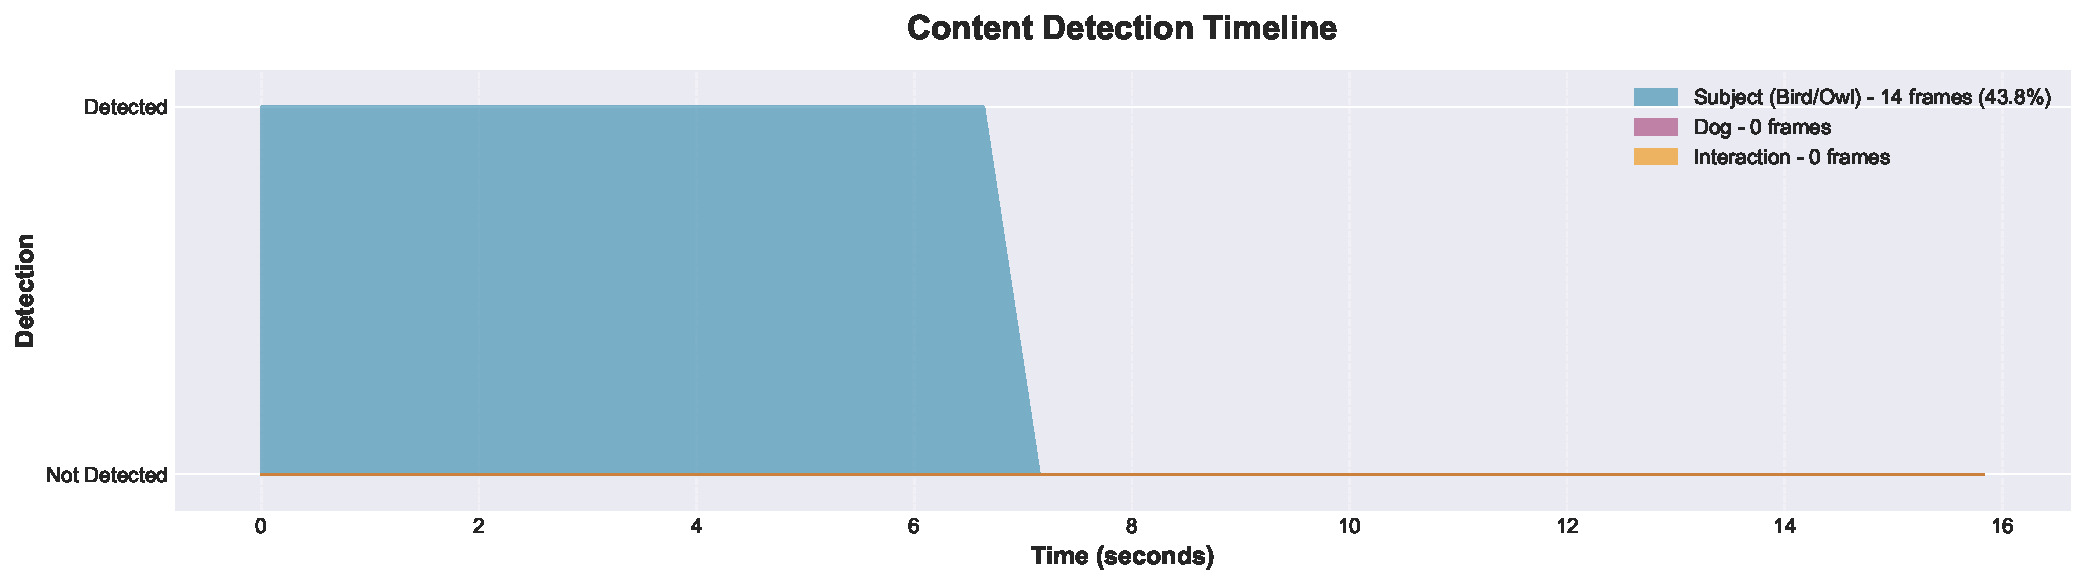
\includegraphics[width=0.7\textwidth]{figures/content_timeline.pdf}
\caption{Subject appears in 14 of 32 analyzed frames (43.8\%), primarily in the first half of the video. Timeline chart showing temporal distribution of subject detection throughout the 15.83-second duration.}
\label{fig-content-timeline}
\end{figure}

\subsection{Event Significance}

This footage documents a rare and historic event: Flaco the owl's first
landing on Fifth Avenue on the night he was freed from the Central Park
Zoo. This represents an important moment in the narrative arc of the
documentary, capturing the first public appearance of Flaco after his
escape.

\needspace{20cm}
\section{Narrative Significance (Story Value)}

\subsection{Narrative Score: 100/100}

\begin{table}[h]
\centering
\small
\caption{Narrative Significance Factors}
\label{tab-narrative-factors}
\begin{tabular}{p{3cm}p{6cm}}
\toprule
\textbf{Factor} & \textbf{Contribution} \\
\midrule
Rare/Unique Event & First-night landing on Fifth Ave \\
Historic Moment & First appearance after zoo escape \\
Subject Visibility & Subject visible in 44\% of footage \\
Multiple-Use Potential & Can be used multiple times throughout documentary \\
Story Importance & High importance \\
\bottomrule
\end{tabular}
\end{table}

\textbf{Multiple-Use Potential:} This footage can be strategically
reused throughout the documentary in:

\begin{table}[h]
\centering
\small
\caption{Multiple-Use Applications}
\label{tab-multiple-use}
\begin{tabular}{p{3.5cm}p{7.5cm}}
\toprule
\textbf{Use Case} & \textbf{Description} \\
\midrule
Opening Sequence & Can be used in documentary opening \\
Transitional Moments & Suitable for scene transitions \\
Key Narrative Scenes & Can feature in important story moments \\
Closing Sequences & Appropriate for documentary conclusion \\
\bottomrule
\end{tabular}
\end{table}

\begin{figure}[h]
\centering
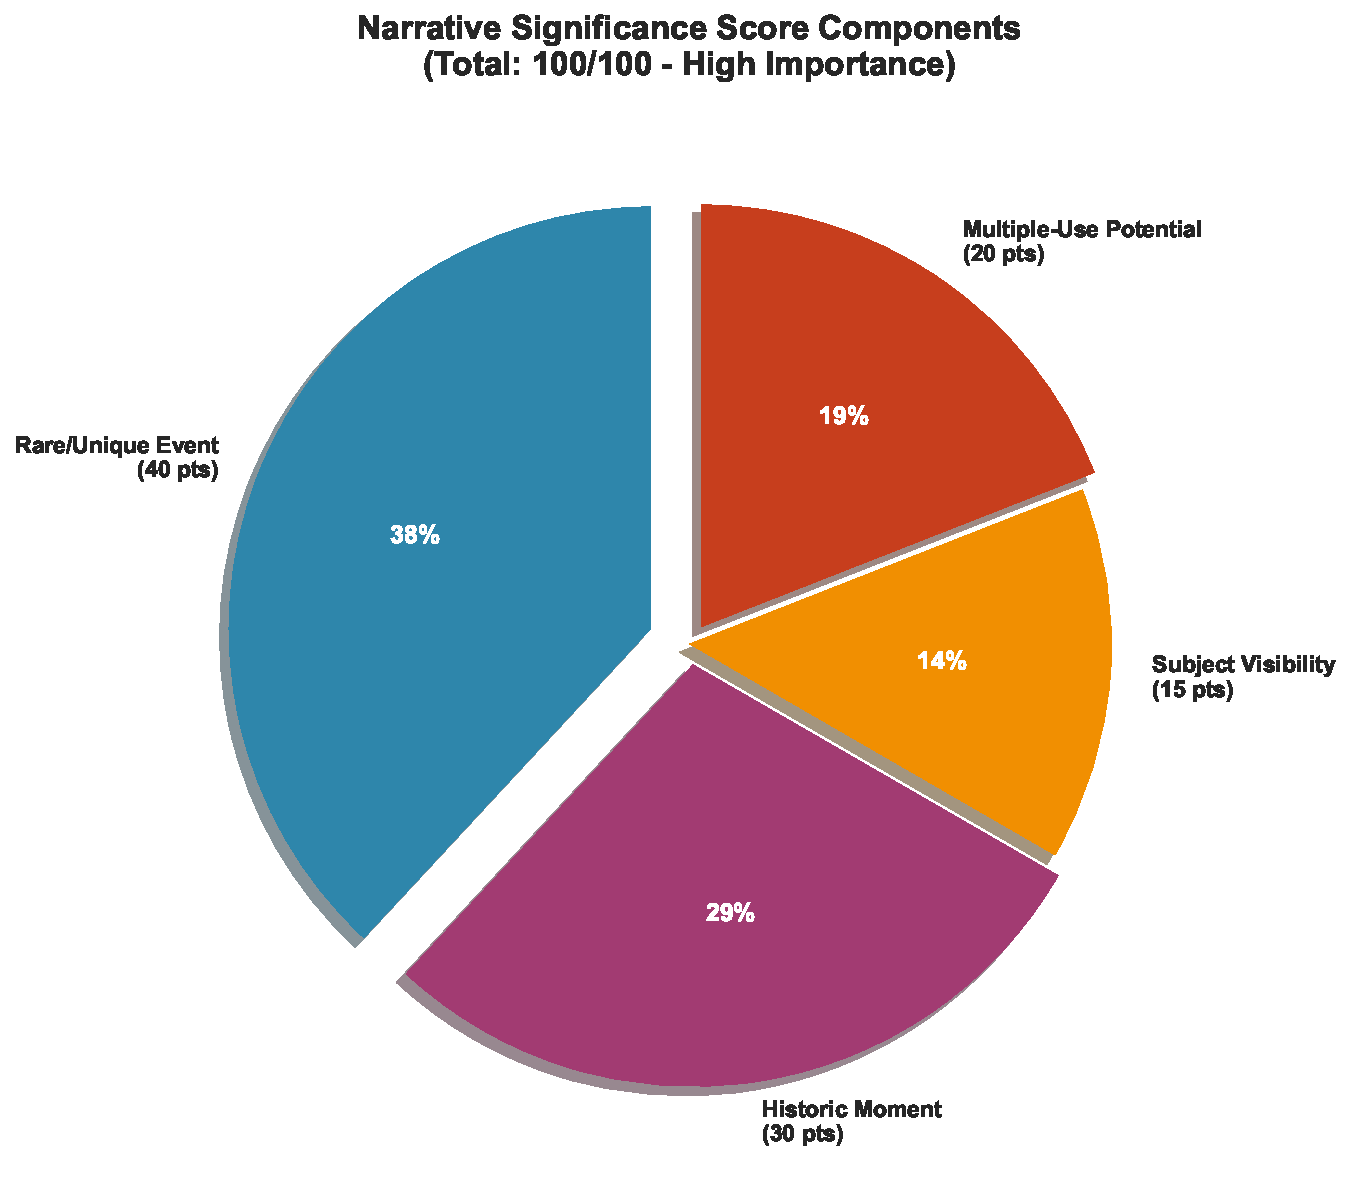
\includegraphics[width=0.5\textwidth]{figures/narrative_significance.pdf}
\caption{High score reflects the footage's importance as a key moment in Flaco's story. Pie chart showing weighted contribution of four factors to narrative significance score of 100/100: Rare/Unique Event (40\%), Historic Moment (30\%), Subject Visibility (15\%) and Multiple-Use Potential (20\%).}
\label{fig-narrative}
\end{figure}

\needspace{25cm}
\section{Usability Analysis}

\subsection{Usability Breakdown}

\begin{figure}[h]
\centering
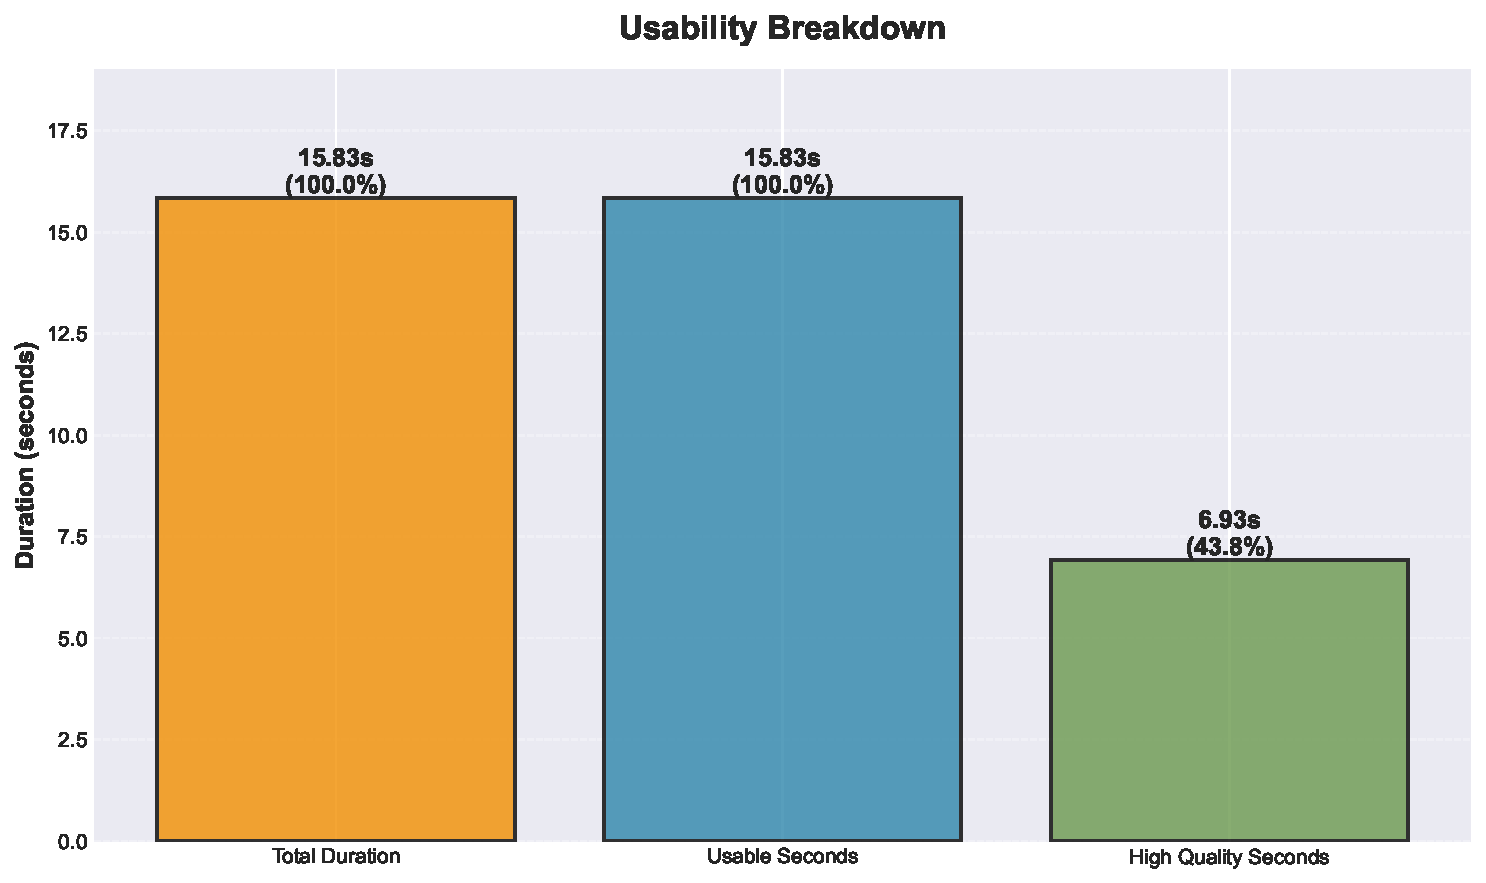
\includegraphics[width=0.7\textwidth]{figures/usability_breakdown.pdf}
\caption{Footage is production-ready with 100\% usability. Bar chart comparing total duration (15.83s, 100\%), usable seconds (15.83s, 100\%) and high-quality seconds (6.93s, 43.8\%).}
\label{fig-usability-breakdown}
\end{figure}

\subsection{Per-Second Breakdown}

\begin{table}[h]
\centering
\small
\caption{Per-Second Breakdown}
\label{tab-per-second}
\begin{tabular}{p{2.5cm}cc}
\toprule
\textbf{Category} & \textbf{Seconds} & \textbf{Percentage} \\
\midrule
Total Duration & 15.83 & 100.0\% \\
Usable Seconds & 15.83 & 100.0\% \\
High Quality Seconds & 6.93 & 43.8\% \\
\bottomrule
\end{tabular}
\end{table}

\textbf{Usable Segments:} 1 continuous segment (0.00s - 15.83s)

\subsection{Clear, Focused Segments}

No continuous clear/focused segments of 1 second or longer were
identified. The footage requires post-processing (sharpening and
stabilization) to achieve optimal clarity for broadcast use.

\needspace{25cm}
\section{Valuation Analysis}

\subsection{Valuation Breakdown}

\begin{figure}[h]
\centering
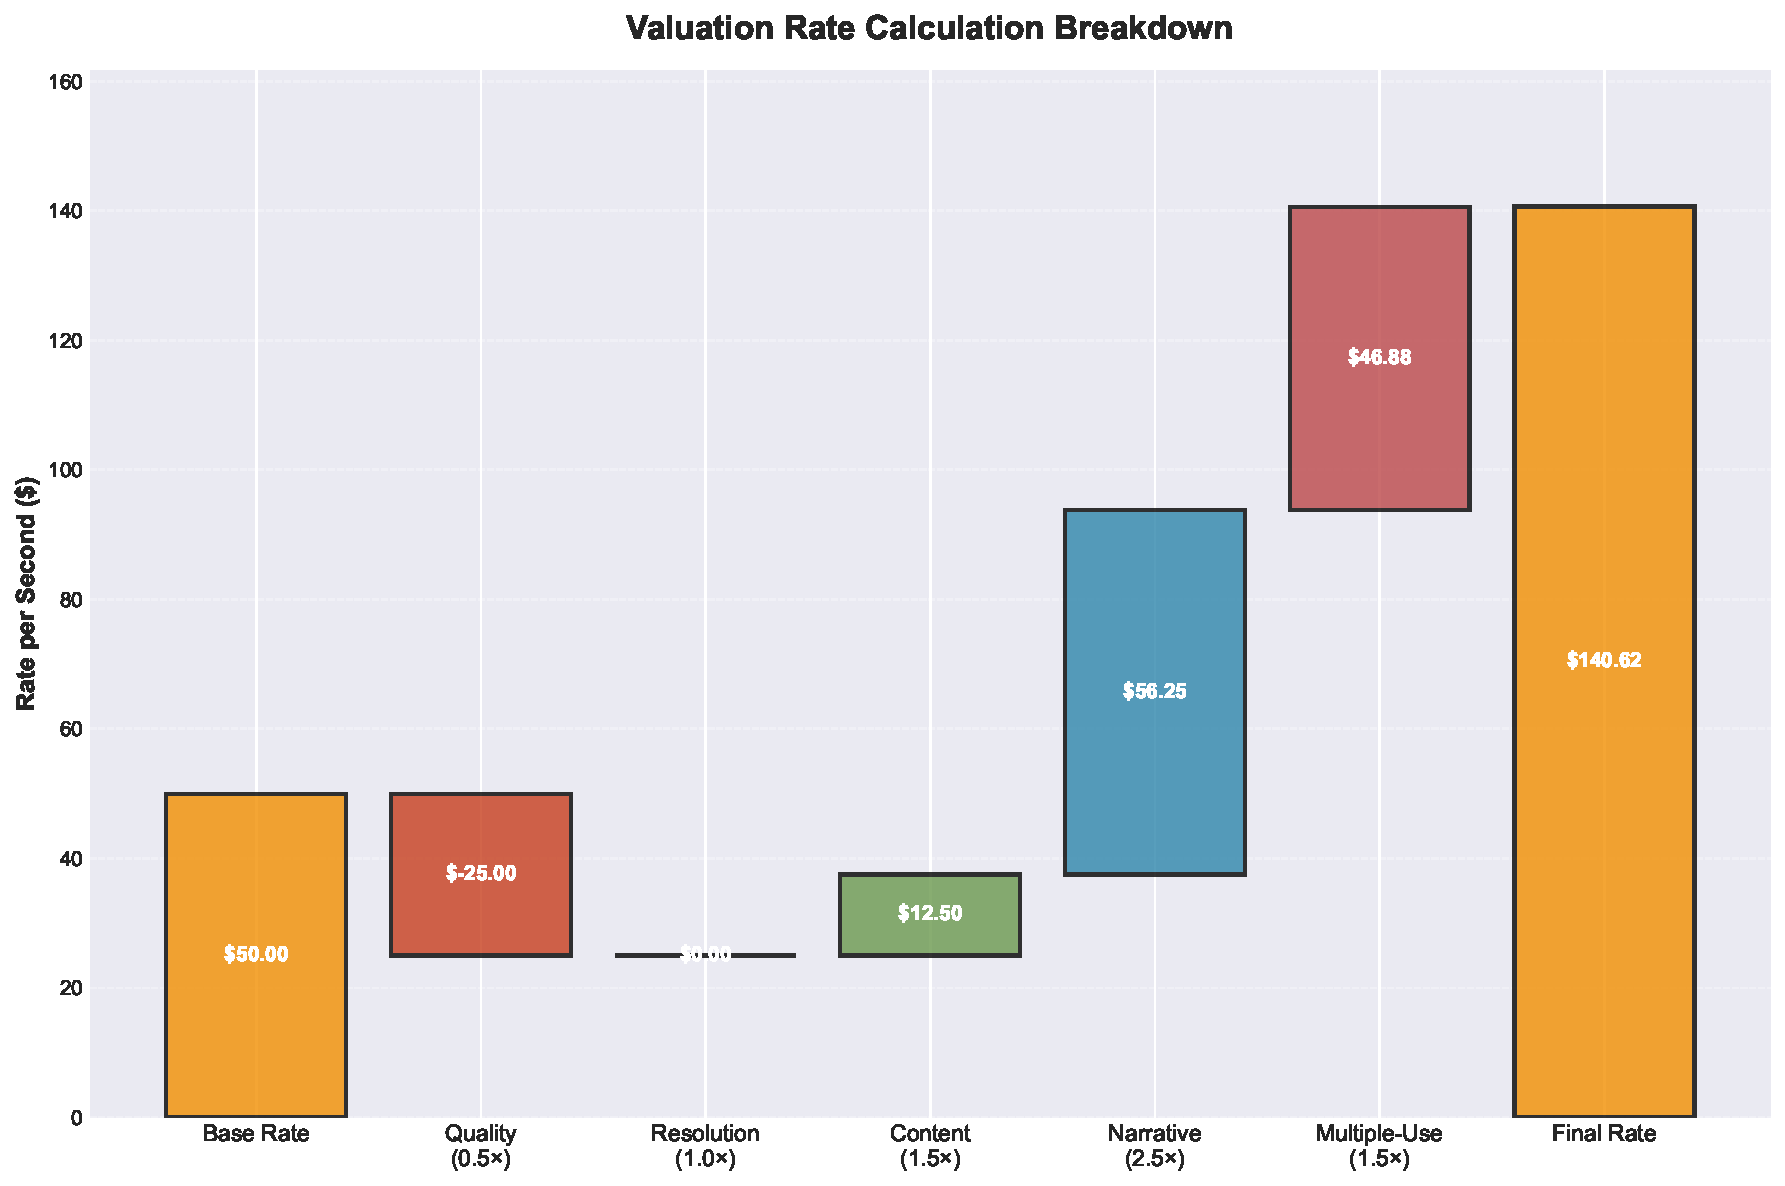
\includegraphics[width=0.75\textwidth]{figures/valuation_breakdown.pdf}
\caption{Final rate \$140.62 per second reflects cumulative effect of all factors. Waterfall chart showing how base rate (\$50.00) is modified by sequential multipliers: Quality (0.50×), Resolution (1.00×), Content Significance (1.50×), Narrative Significance (2.50×) and Multiple-Use (1.50×).}
\label{fig-valuation-breakdown}
\end{figure}

\needspace{8cm}
\subsection{Rate Calculation}

\enlargethispage{2cm}
\vspace{-0.5cm}
\begin{table}[H]
\centering
\footnotesize
\caption{Rate Calculation}
\label{tab-rate-calculation}
\begin{tabular}{p{3.5cm}p{1.8cm}p{4.2cm}}
\toprule
\textbf{Factor} & \textbf{Multiplier} & \textbf{Value} \\
\midrule
Base Rate (per usable second) & 1.00× & \$50.00 \\
Quality Multiplier & 0.50× & \\
Resolution Multiplier & 1.00× & \\
Content Significance Multiplier & 1.50× & \\
Narrative Significance Multiplier & 2.50× & \\
Multiple-Use Multiplier & 1.50× & \\
\textbf{Final Rate per Second} & & \textbf{\$140.62} \\
\bottomrule
\end{tabular}
\end{table}

\needspace{8cm}
\subsection{Estimated Value Range}

\begin{table}[h]
\centering
\small
\caption{Estimated Value Range}
\label{tab-value-range}
\begin{tabular}{p{3cm}p{5cm}p{3cm}}
\toprule
\textbf{Estimate Type} & \textbf{Calculation} & \textbf{Value} \\
\midrule
Conservative & All usable seconds × \$140.62 & \$2,226 \\
Optimistic & Premium segments at 1.5× rate & \$2,713 \\
\textbf{Recommended Range} & & \textbf{\$2,226 - \$2,713} \\
\bottomrule
\end{tabular}
\end{table}

\needspace{12cm}
\subsection{Value Factors}

\begin{table}[h]
\centering
\small
\caption{Value Factors}
\label{tab-value-factors}
\begin{tabular}{p{3cm}p{7cm}}
\toprule
\textbf{Factor} & \textbf{Description} \\
\midrule
Usability & High usability (100\% usable) - most of the clip is production-ready \\
Archival Value & Rare/unique event adds archival and narrative value \\
Story Value & Story moment with reuse potential increases value \\
Multiple-Use & Footage can be used multiple times throughout documentary structure \\
\bottomrule
\end{tabular}
\end{table}

\section{Conclusion}

This footage represents an important moment in Flaco the owl's story,
documenting his first landing on Fifth Avenue after being freed from the
Central Park Zoo. While the technical quality requires post-processing,
the narrative significance, rarity and multiple-use potential make this
footage valuable for documentary production.

The estimated licensing value range of \$2,226 - \$2,713 reflects both
the technical quality considerations and the narrative value of this
historic moment.



\end{document}
